\section{Model predictions errors for counties in the United States}

% ERRORS

\begin{landscape}
\begin{table}[!htb]
    \centering
    \begin{tabular}{| c | c | c | c | c | c | c | c | c | c | c |}
        \multirow{2}{*}{Days}
            & \multirow{2}{*}{Loc.}
            & \multicolumn{3}{c |}{Baseline}
            & \multicolumn{3}{c |}{2nd. Ver}
            & \multicolumn{3}{c |}{3rd. Ver} \\ \cline{3-11}
            & & MAE & MAPE & RMSE & MAE & MAPE & RMSE & MAE & MAPE & RMSE \\ \hline\hline

        \multirow{4}{*}{7}
            & Cook, IL & \textbf{5.847} & \textbf{0.055} & \textbf{6.291} & 18.390 & 0.173 & 19.257 & 21.309 & 0.200 & 22.031 \\ \cline{2-11}
            & Harris, TX & 46.021 & 0.666 & 50.000 & 38.705 & 0.560 & 43.120 & \textbf{32.571} & \textbf{0.471} & \textbf{36.267} \\ \cline{2-11}
            & Los Angeless, CA & \textbf{28.781} & \textbf{0.115} & \textbf{31.633} & 51.605 & 0.206 & 54.813 & 50.488 & 0.202 & 53.633 \\ \cline{2-11}
            & Maricopa, AZ & 39.739 & 0.374 & 40.227 & 38.180 & 0.360 & 38.746 & \textbf{36.632} & \textbf{0.345} & \textbf{37.215} \\ \hline

        \multirow{4}{*}{14}
            & Cook, IL & \textbf{13.181} & \textbf{0.123} & \textbf{15.800} & 31.772 & 0.297 & 35.375 & 34.551 & 0.323 & 37.832 \\ \cline{2-11}
            & Harris, TX & 95.339 & 1.355 & 111.180 & 87.944 & 1.249 & 104.920 & \textbf{74.100} & \textbf{1.052} & \textbf{88.397} \\ \cline{2-11}
            & Los Angeless, CA & \textbf{54.539} & \textbf{0.217} & \textbf{61.814} & 87.975 & 0.350 & 97.176 & 86.045 & 0.343 & 95.029 \\ \cline{2-11}
            & Maricopa, AZ & 55.439 & 0.519 & 58.393 & 54.897 & 0.514 & 58.269 & \textbf{53.215} & \textbf{0.498} & \textbf{56.632} \\ \hline

        \multirow{4}{*}{21}
            & Cook, IL & \textbf{21.380} & \textbf{0.199} & \textbf{25.491} & 45.720 & 0.426 & 51.581 & 48.620 & 0.453 & 54.215 \\ \cline{2-11}
            & Harris, TX & 158.343 & 2.205 & 189.162 & 152.570 & 2.123 & 185.661 & \textbf{127.313} & \textbf{1.772} & \textbf{154.368} \\ \cline{2-11}
            & Los Angeless, CA & \textbf{82.513} & \textbf{0.327} & \textbf{95.410} & 126.976 & 0.503 & 143.413 & 123.921 & 0.491 & 139.857 \\ \cline{2-11}
            & Maricopa, AZ & 76.472 & 0.711 & \textbf{83.882} & 77.590 & 0.721 & 86.019 & \textbf{75.672} & \textbf{0.703} & 84.128 \\ \hline

        \multirow{4}{*}{28}
            & Cook, IL & \textbf{29.629} & \textbf{0.275} & \textbf{35.088} & 59.121 & 0.549 & 66.872 & 62.355 & 0.579 & 69.979 \\ \cline{2-11}
            & Harris, TX & 227.124 & 3.099 & 272.682 & 225.190 & 3.070 & 274.928 & \textbf{184.261} & \textbf{2.513} & \textbf{223.061} \\ \cline{2-11}
            & Los Angeless, CA & \textbf{117.110} & \textbf{0.461} & \textbf{138.626} & 171.721 & 0.677 & 197.699 & 167.210 & 0.659 & 192.284 \\ \cline{2-11}
            & Maricopa, AZ & \textbf{101.192} & \textbf{0.933} & \textbf{114.101} & 104.663 & 0.965 & 119.408 & 102.385 & 0.944 & 117.066 \\ \hline
    \end{tabular}
    \caption{Out-of-sample errors of the model's predictions on the number of deaths for the counties in the United States. The lowest errors for each evaluation metrics at each location are highlighted.}
\end{table}
\end{landscape}

\begin{landscape}
\begin{table}[!htb]
    \centering
    \begin{tabular}{| c | c | c | c | c | c | c | c | c | c | c |}
        \multirow{2}{*}{Days}
            & \multirow{2}{*}{Loc.}
            & \multicolumn{3}{c |}{Baseline}
            & \multicolumn{3}{c |}{2nd. Ver}
            & \multicolumn{3}{c |}{3rd. Ver} \\ \cline{3-11}
            & & MAE & MAPE & RMSE & MAE & MAPE & RMSE & MAE & MAPE & RMSE \\ \hline\hline

        \multirow{4}{*}{7}
            & Cook, IL & \textbf{22.545} & \textbf{2.377} & \textbf{28.432} & 55.668 & 6.041 & 66.778 & 41.352 & 4.467 & 55.134 \\ \cline{2-11}
            & Harris, TX & 1022.438 & 30.850 & 1193.354 & 1093.142 & 32.772 & 1280.746 & \textbf{797.754} & \textbf{26.782} & \textbf{865.731} \\ \cline{2-11}
            & Los Angeless, CA & \textbf{981.461} & \textbf{20.945} & \textbf{1140.886} & 1126.805 & 24.141 & 1297.286 & 1082.929 & 23.181 & 1248.996 \\ \cline{2-11}
            & Maricopa, AZ & 95.129 & 4.730 & 99.906 & 19.956 & 0.987 & 23.867 & \textbf{19.382} & \textbf{0.968} & \textbf{21.617} \\ \hline

        \multirow{4}{*}{14}
            & Cook, IL & \textbf{35.341} & \textbf{3.517} & \textbf{45.173} & 90.017 & 9.156 & 101.192 & 59.667 & 6.104 & 68.594 \\ \cline{2-11}
            & Harris, TX & 890.257 & \textbf{28.652} & 1093.096 & 984.436 & 30.810 & 1205.333 & \textbf{790.239} & 30.445 & \textbf{874.964} \\ \cline{2-11}
            & Los Angeless, CA & \textbf{698.901} & \textbf{15.302} & \textbf{950.789} & 802.626 & 17.610 & 1085.485 & 768.943 & 16.918 & 1038.125 \\ \cline{2-11}
            & Maricopa, AZ & 136.129 & 6.883 & 172.143 & 69.022 & 3.427 & \textbf{94.846} & \textbf{62.939} & \textbf{3.176} & 95.737 \\ \hline

        \multirow{4}{*}{21}
            & Cook, IL & \textbf{70.168} & \textbf{7.131} & \textbf{92.661} & 136.784 & 14.489 & 177.086 & 96.828 & 10.550 & 144.579 \\ \cline{2-11}
            & Harris, TX & 715.160 & \textbf{23.718} & 932.114 & 963.073 & 32.888 & 1132.567 & \textbf{671.354} & 26.827 & \textbf{775.119} \\ \cline{2-11}
            & Los Angeless, CA & \textbf{477.179} & \textbf{10.682} & \textbf{776.682} & 557.786 & 12.785 & 887.881 & 584.712 & 14.463 & 857.916 \\ \cline{2-11}
            & Maricopa, AZ & 139.674 & 6.888 & 169.314 & 92.801 & 4.357 & 129.381 & \textbf{76.112} & \textbf{3.609} & \textbf{116.774} \\ \hline

        \multirow{4}{*}{28}
            & Cook, IL & \textbf{83.696} & \textbf{8.105} & \textbf{119.396} & 184.792 & 19.135 & 230.863 & 139.144 & 14.665 & 190.726 \\ \cline{2-11}
            & Harris, TX & \textbf{605.536} & \textbf{20.796} & 824.160 & 982.211 & 35.537 & 1123.076 & 689.374 & 28.746 & \textbf{779.813} \\ \cline{2-11}
            & Los Angeless, CA & \textbf{412.908} & \textbf{11.617} & \textbf{686.484} & 498.917 & 14.897 & 794.109 & 546.785 & 17.824 & 784.312 \\ \cline{2-11}
            & Maricopa, AZ & 217.947 & 11.510 & 271.885 & \textbf{104.125} & \textbf{5.223} & \textbf{134.620} & 109.935 & 5.689 & 149.951 \\ \hline
    \end{tabular}
    \caption{Out-of-sample errors of the model's predictions on the number of new cases for the counties in the United States. The lowest errors for each evaluation metrics at each location are highlighted.}
\end{table}
\end{landscape}

\begin{landscape}
\begin{table}[!htb]
    \centering
    \begin{tabular}{| c | c | c | c | c | c | c | c | c | c | c |}
        \multirow{2}{*}{Days}
            & \multirow{2}{*}{Loc.}
            & \multicolumn{3}{c |}{Baseline}
            & \multicolumn{3}{c |}{2nd. Ver}
            & \multicolumn{3}{c |}{3rd. Ver} \\ \cline{3-11}
            & & MAE & MAPE & RMSE & MAE & MAPE & RMSE & MAE & MAPE & RMSE \\ \hline\hline

        \multirow{4}{*}{7}
            & Cook, IL & 678.757 & 0.117 & 679.641 & 750.786 & 0.130 & 761.605 & \textbf{595.890} & \textbf{0.103} & \textbf{604.919} \\ \cline{2-11}
            & Harris, TX & 2429.798 & 0.520 & 3193.800 & 2629.532 & 0.562 & 3482.363 & \textbf{1535.176} & \textbf{0.333} & \textbf{1736.348} \\ \cline{2-11}
            & Los Angeless, CA & \textbf{2351.443} & \textbf{0.172} & \textbf{2920.659} & 2898.771 & 0.212 & 3633.093 & 2545.519 & 0.186 & 3107.429 \\ \cline{2-11}
            & Maricopa, AZ & 1491.513 & 0.242 & 1510.229 & 974.924 & 0.159 & 975.073 & \textbf{410.099} & \textbf{0.067} & \textbf{412.091} \\ \hline

        \multirow{4}{*}{14}
            & Cook, IL & \textbf{612.953} & \textbf{0.105} & \textbf{621.265} & 1129.956 & 0.194 & 1212.272 & 874.273 & 0.150 & 928.652 \\ \cline{2-11}
            & Harris, TX & 5883.932 & 1.224 & 6993.098 & 6824.524 & 1.419 & 8209.270 & \textbf{2209.289} & \textbf{0.465} & \textbf{2506.827} \\ \cline{2-11}
            & Los Angeless, CA & \textbf{5141.081} & \textbf{0.371} & \textbf{5985.620} & 6376.008 & 0.460 & 7440.514 & 5501.848 & 0.397 & 6381.884 \\ \cline{2-11}
            & Maricopa, AZ & 2026.365 & 0.325 & 2112.334 & 963.663 & 0.155 & 969.336 & \textbf{480.406} & \textbf{0.077} & \textbf{492.111} \\ \hline

        \multirow{4}{*}{21}
            & Cook, IL & \textbf{465.474} & \textbf{0.080} & \textbf{519.420} & 1659.534 & 0.282 & 1879.133 & 1219.233 & 0.207 & 1359.485 \\ \cline{2-11}
            & Harris, TX & 7611.514 & 1.553 & 8583.826 & 9913.906 & 2.017 & 11519.766 & \textbf{1664.322} & \textbf{0.348} & \textbf{2097.628} \\ \cline{2-11}
            & Los Angeless, CA & \textbf{6242.229} & \textbf{0.447} & \textbf{6903.758} & 7690.419 & 0.551 & 8509.198 & 6313.624 & 0.452 & 6943.113 \\ \cline{2-11}
            & Maricopa, AZ & 2549.187 & 0.402 & 2705.335 & 767.923 & 0.123 & 826.909 & \textbf{396.265} & \textbf{0.063} & \textbf{425.505} \\ \hline

        \multirow{4}{*}{28}
            & Cook, IL & \textbf{486.965} & \textbf{0.083} & \textbf{548.673} & 2493.195 & 0.420 & 3000.083 & 1869.379 & 0.315 & 2260.015 \\ \cline{2-11}
            & Harris, TX & 8785.001 & 1.760 & 9652.091 & 13119.518 & 2.612 & 15167.205 & \textbf{2479.698} & \textbf{0.499} & \textbf{3145.165} \\ \cline{2-11}
            & Los Angeless, CA & 6715.207 & 0.478 & 7232.734 & 7974.478 & 0.568 & 8596.755 & \textbf{6094.396} & \textbf{0.435} & \textbf{6615.172} \\ \cline{2-11}
            & Maricopa, AZ & 3327.537 & 0.517 & 3705.984 & 670.792 & 0.107 & 754.504 & \textbf{452.858} & \textbf{0.071} & \textbf{533.121} \\ \hline
    \end{tabular}
    \caption{Out-of-sample errors of the model's predictions on the number of cumulative cases for the counties in the United States. The lowest errors for each evaluation metrics at each location are highlighted.}
\end{table}
\end{landscape}

\subsection{Reproduction number and fatality rate}

\begin{figure}[!htb]
    \centering

    \begin{subfigure}[b]{\linewidth}
        \centering
        \begin{subfigure}[b]{0.4\linewidth}
            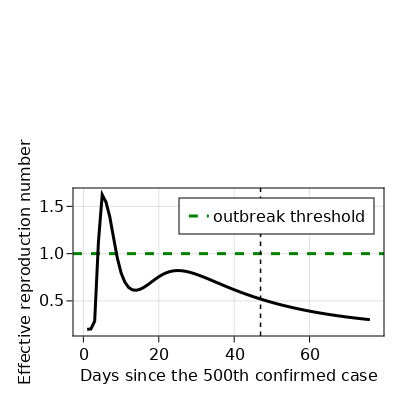
\includegraphics[width=\linewidth]{baseline/cook_il/20211215163025.baseline.cook_il.R_effective.png}
        \end{subfigure}
        \begin{subfigure}[b]{0.4\linewidth}
            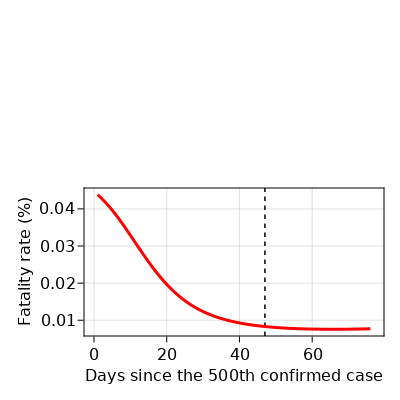
\includegraphics[width=\linewidth]{baseline/cook_il/20211215163025.baseline.cook_il.fatality_rate.png}
        \end{subfigure}
        \subcaption{Baseline model}
    \end{subfigure}

    \begin{subfigure}[b]{\linewidth}
        \centering
        \begin{subfigure}[b]{0.4\linewidth}
            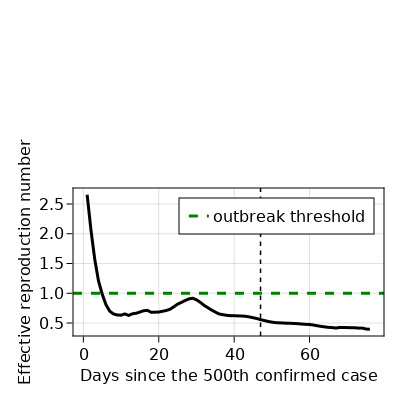
\includegraphics[width=\linewidth]{fb1/cook_il/20211216131821.fbmobility1.cook_il.R_effective.png}
        \end{subfigure}
        \begin{subfigure}[b]{0.4\linewidth}
            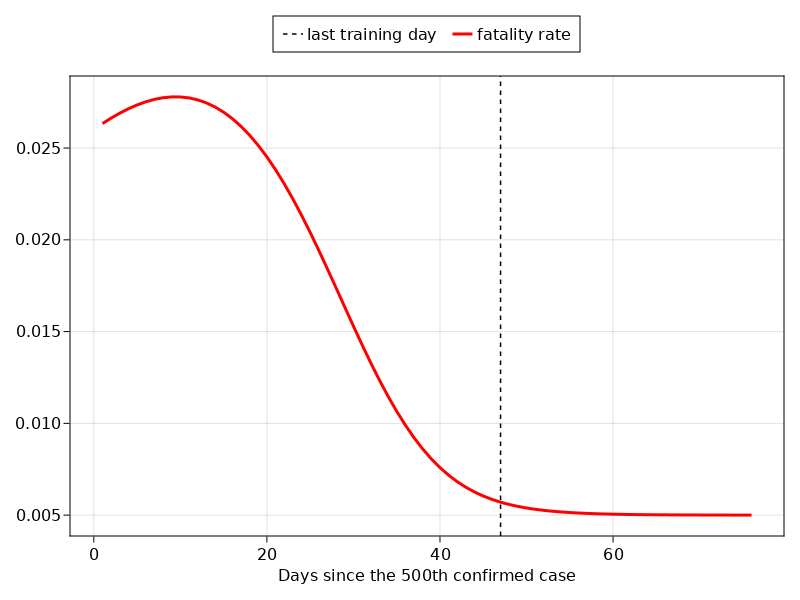
\includegraphics[width=\linewidth]{fb1/cook_il/20211216131821.fbmobility1.cook_il.fatality_rate.png}
        \end{subfigure}
        \subcaption{2nd. version}
    \end{subfigure}

    \begin{subfigure}[b]{\linewidth}
        \centering
        \begin{subfigure}[b]{0.4\linewidth}
            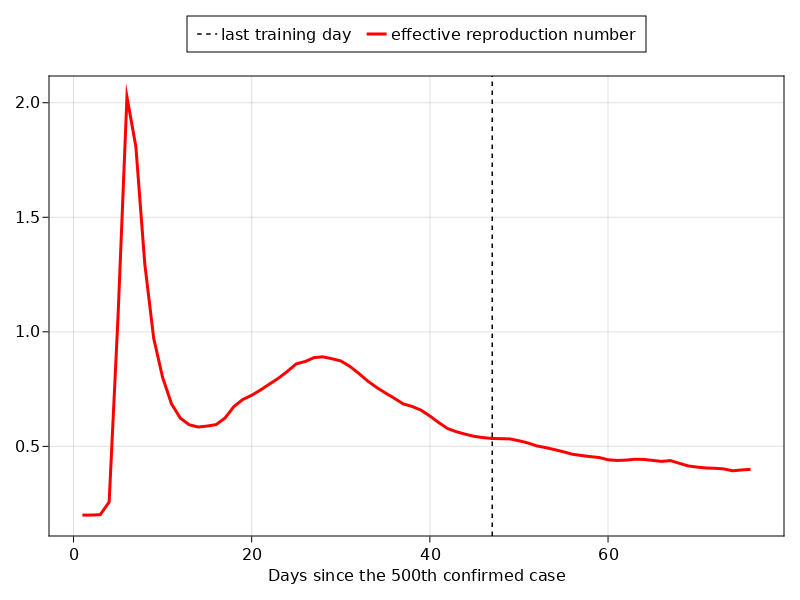
\includegraphics[width=\linewidth]{fb2/cook_il/20211216142727.fbmobility2.cook_il.R_effective.png}
        \end{subfigure}
        \begin{subfigure}[b]{0.4\linewidth}
            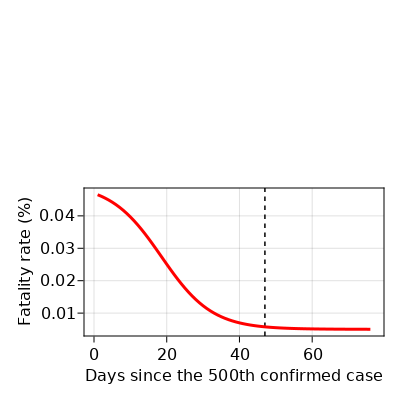
\includegraphics[width=\linewidth]{fb2/cook_il/20211216142727.fbmobility2.cook_il.fatality_rate.png}
        \end{subfigure}
        \subcaption{3rd. version}
    \end{subfigure}

    \caption{The effective reproduction number and the fatality rate for Cook (Illinois), learned by different versions of the model}
    \label{fig:R0-and-fatality-cook}
\end{figure}

\begin{figure}[!htb]
    \centering

    \begin{subfigure}[b]{\linewidth}
        \centering
        \begin{subfigure}[b]{0.4\linewidth}
            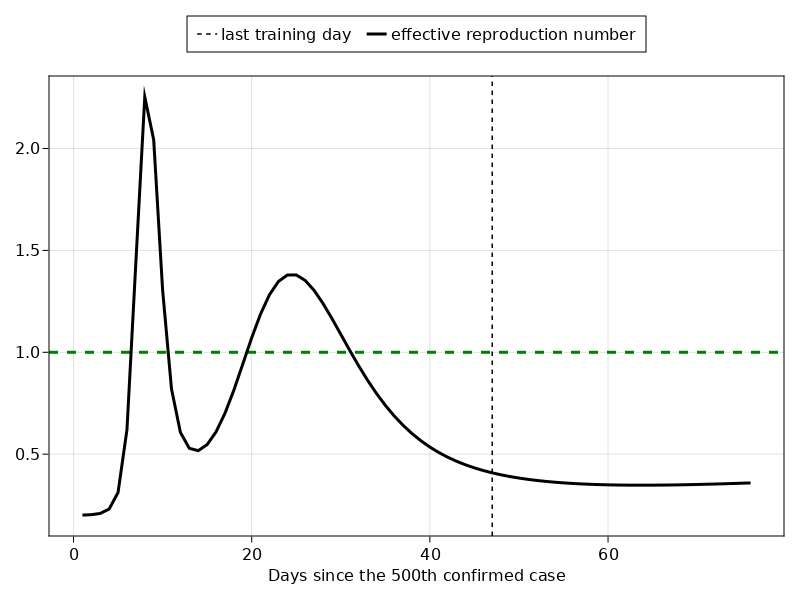
\includegraphics[width=\linewidth]{baseline/harris_tx/20211216154445.baseline.harris_tx.R_effective.png}
        \end{subfigure}
        \begin{subfigure}[b]{0.4\linewidth}
            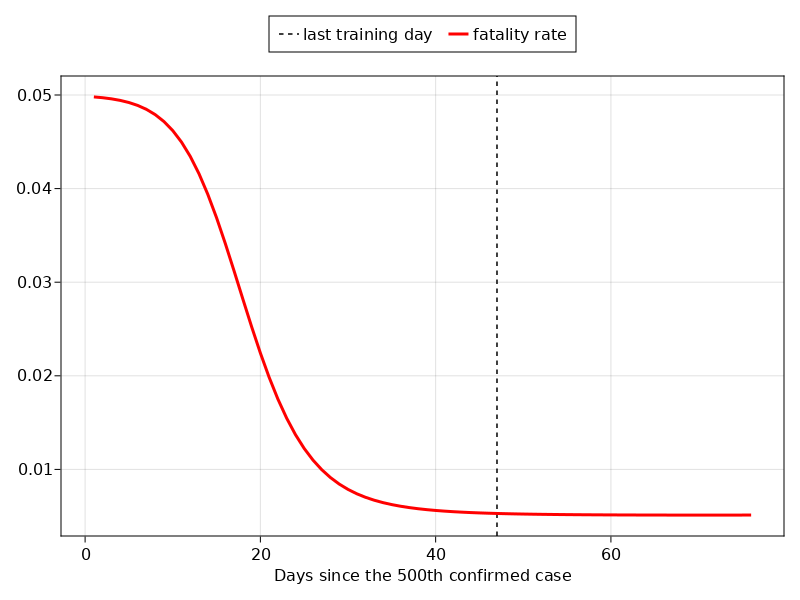
\includegraphics[width=\linewidth]{baseline/harris_tx/20211216154445.baseline.harris_tx.fatality_rate.png}
        \end{subfigure}
        \subcaption{Baseline model}
    \end{subfigure}

    \begin{subfigure}[b]{\linewidth}
        \centering
        \begin{subfigure}[b]{0.4\linewidth}
            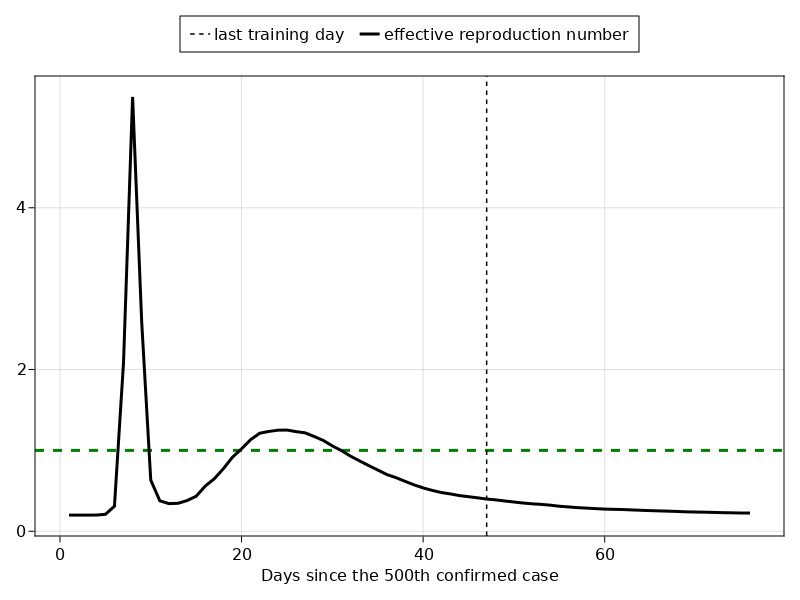
\includegraphics[width=\linewidth]{fb1/harris_tx/20211216231719.fbmobility1.harris_tx.R_effective.png}
        \end{subfigure}
        \begin{subfigure}[b]{0.4\linewidth}
            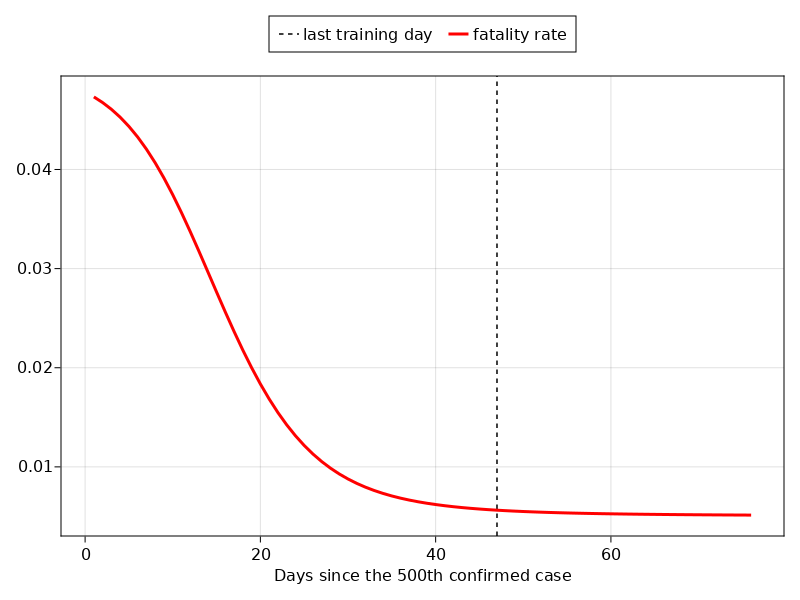
\includegraphics[width=\linewidth]{fb1/harris_tx/20211216231719.fbmobility1.harris_tx.fatality_rate.png}
        \end{subfigure}
        \subcaption{2nd. version}
    \end{subfigure}

    \begin{subfigure}[b]{\linewidth}
        \centering
        \begin{subfigure}[b]{0.4\linewidth}
            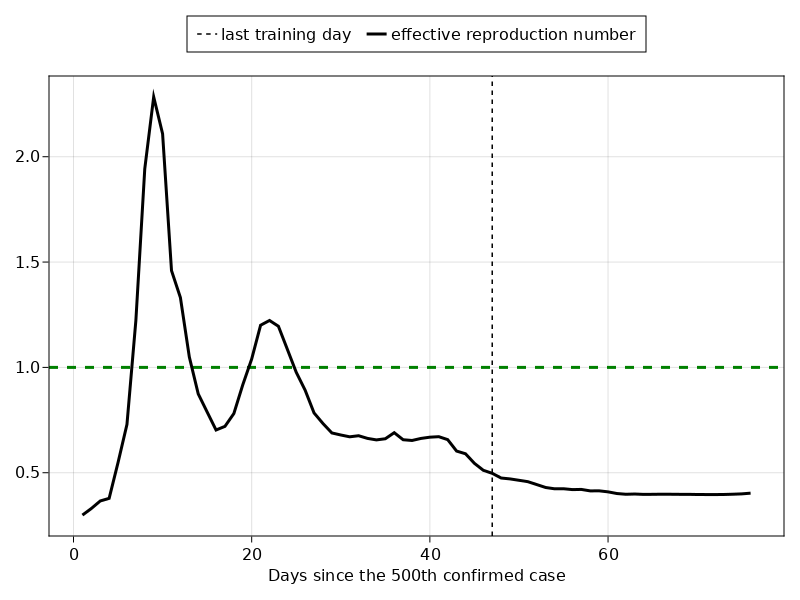
\includegraphics[width=\linewidth]{fb2/harris_tx/20211217204936.fbmobility2.harris_tx.R_effective.png}
        \end{subfigure}
        \begin{subfigure}[b]{0.4\linewidth}
            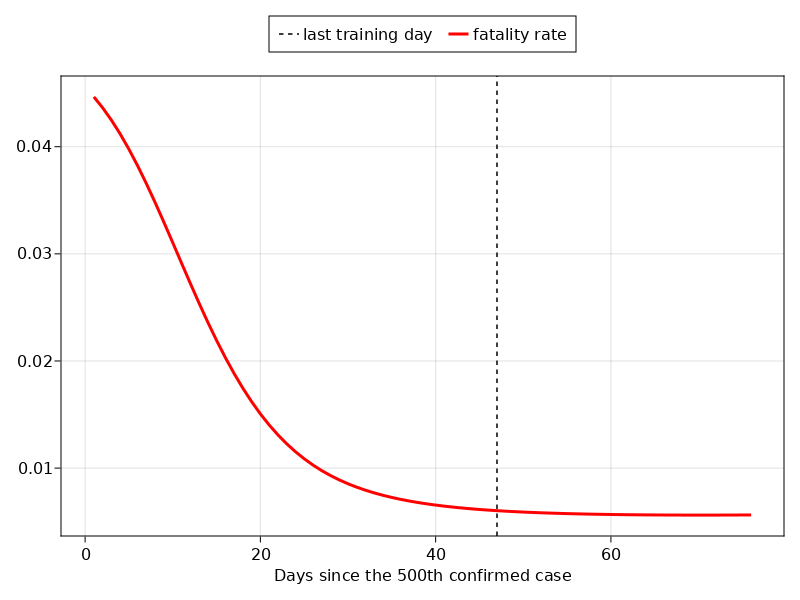
\includegraphics[width=\linewidth]{fb2/harris_tx/20211217204936.fbmobility2.harris_tx.fatality_rate.png}
        \end{subfigure}
        \subcaption{3rd. version}
    \end{subfigure}

    \caption{The effective reproduction number and the fatality rate for Harris (Texas) learned by different versions of the model}
    \label{fig:R0-and-fatality-harris}
\end{figure}


\begin{figure}[!htb]
    \centering

    \begin{subfigure}[b]{\linewidth}
        \centering
        \begin{subfigure}[b]{0.4\linewidth}
            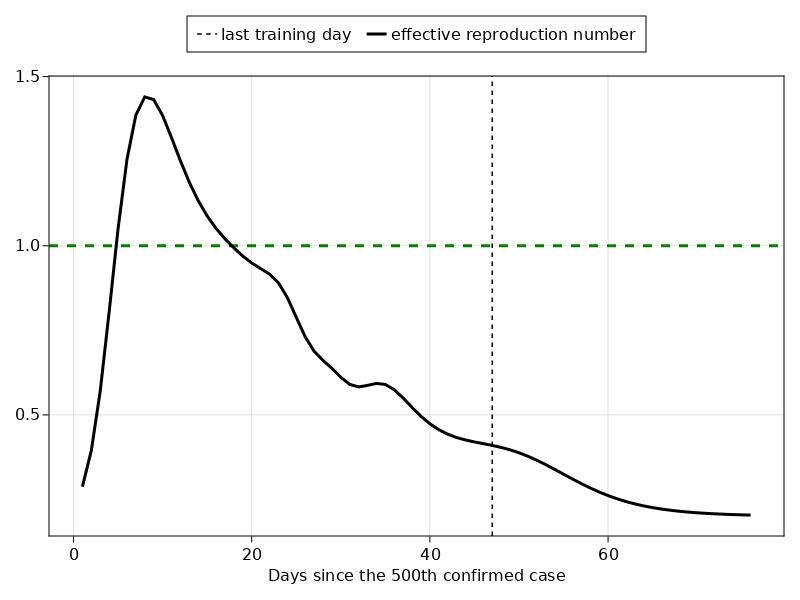
\includegraphics[width=\linewidth]{baseline/losangeles_ca/20211216124108.baseline.losangeles_ca.R_effective.png}
        \end{subfigure}
        \begin{subfigure}[b]{0.4\linewidth}
            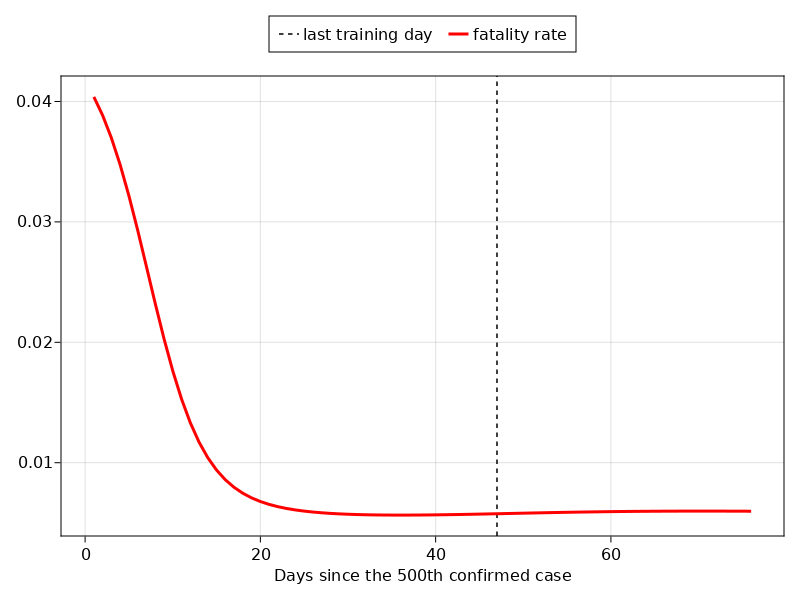
\includegraphics[width=\linewidth]{baseline/losangeles_ca/20211216124108.baseline.losangeles_ca.fatality_rate.png}
        \end{subfigure}
        \subcaption{Baseline model}
    \end{subfigure}

    \begin{subfigure}[b]{\linewidth}
        \centering
        \begin{subfigure}[b]{0.4\linewidth}
            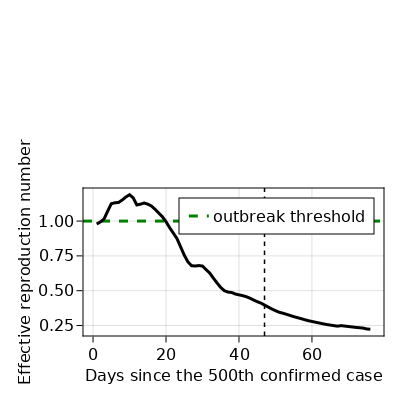
\includegraphics[width=\linewidth]{fb1/losangeles_ca/20211216180602.fbmobility1.losangeles_ca.R_effective.png}
        \end{subfigure}
        \begin{subfigure}[b]{0.4\linewidth}
            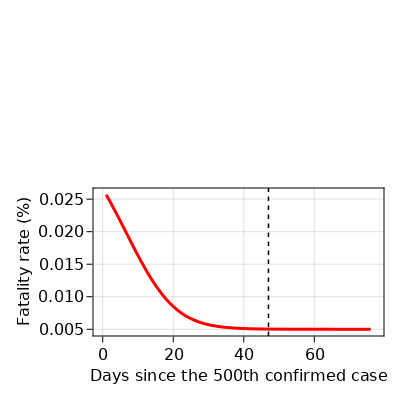
\includegraphics[width=\linewidth]{fb1/losangeles_ca/20211216180602.fbmobility1.losangeles_ca.fatality_rate.png}
        \end{subfigure}
        \subcaption{2nd. version}
    \end{subfigure}

    \begin{subfigure}[b]{\linewidth}
        \centering
        \begin{subfigure}[b]{0.4\linewidth}
            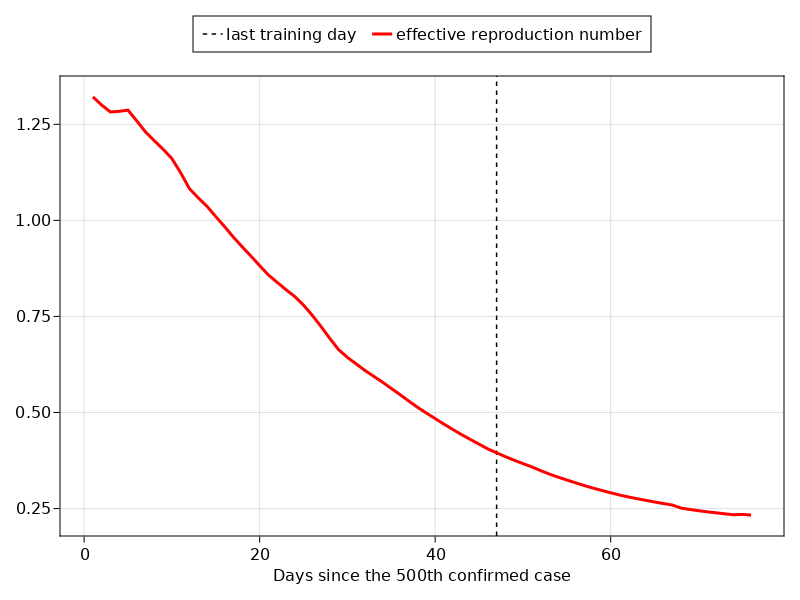
\includegraphics[width=\linewidth]{fb2/losangeles_ca/20211216142727.fbmobility2.losangeles_ca.R_effective.png}
        \end{subfigure}
        \begin{subfigure}[b]{0.4\linewidth}
            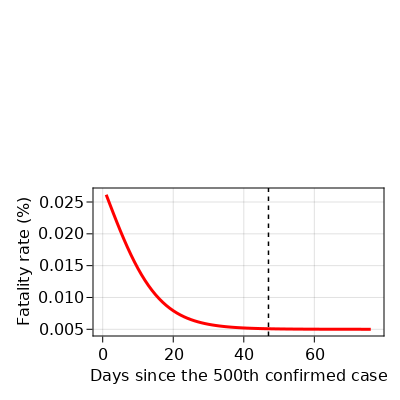
\includegraphics[width=\linewidth]{fb2/losangeles_ca/20211216142727.fbmobility2.losangeles_ca.fatality_rate.png}
        \end{subfigure}
        \subcaption{3rd. version}
    \end{subfigure}

    \caption{The effective reproduction number and the fatality rate for Los Angeles (California) learned by different versions of the model}
    \label{fig:R0-and-fatality-losangeles}
\end{figure}

\begin{figure}[!htb]
    \centering

    \begin{subfigure}[b]{\linewidth}
        \centering
        \begin{subfigure}[b]{0.4\linewidth}
            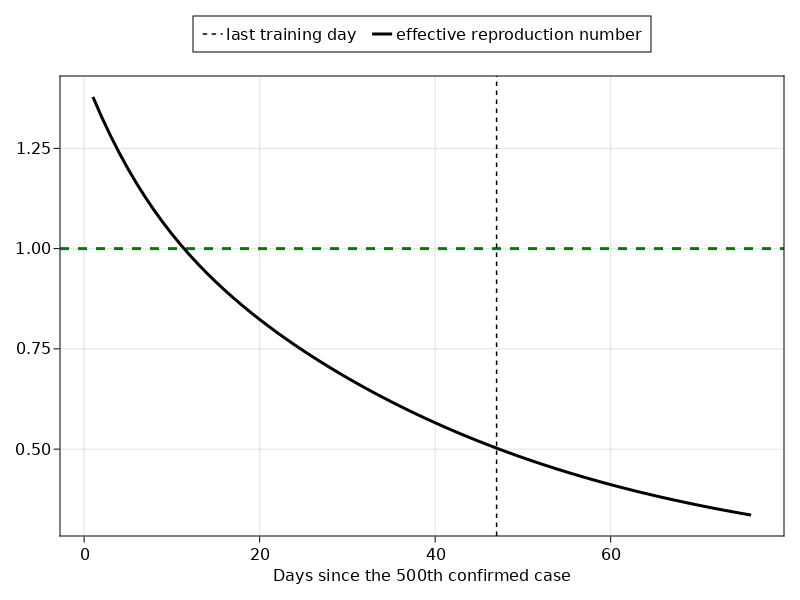
\includegraphics[width=\linewidth]{baseline/maricopa_az/20211216154445.baseline.maricopa_az.R_effective.png}
        \end{subfigure}
        \begin{subfigure}[b]{0.4\linewidth}
            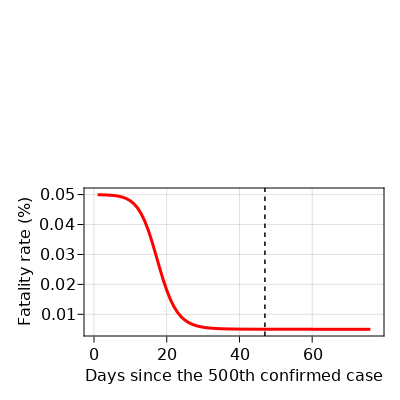
\includegraphics[width=\linewidth]{baseline/maricopa_az/20211216154445.baseline.maricopa_az.fatality_rate.png}
        \end{subfigure}
        \subcaption{Baseline model}
    \end{subfigure}

    \begin{subfigure}[b]{\linewidth}
        \centering
        \begin{subfigure}[b]{0.4\linewidth}
            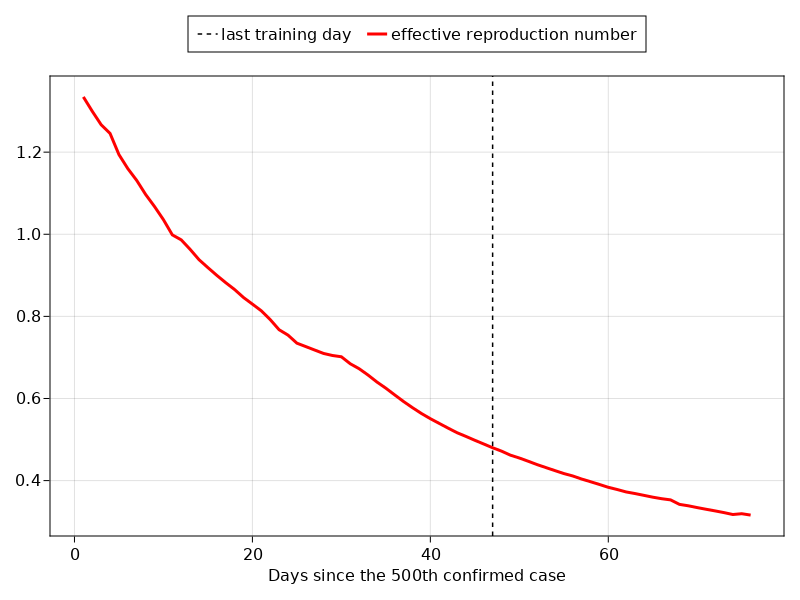
\includegraphics[width=\linewidth]{fb1/maricopa_az/20211216131821.fbmobility1.maricopa_az.R_effective.png}
        \end{subfigure}
        \begin{subfigure}[b]{0.4\linewidth}
            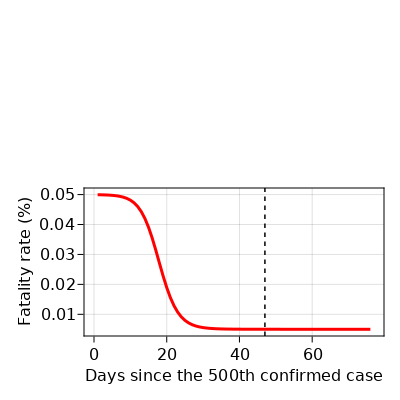
\includegraphics[width=\linewidth]{fb1/maricopa_az/20211216131821.fbmobility1.maricopa_az.fatality_rate.png}
        \end{subfigure}
        \subcaption{2nd. version}
    \end{subfigure}

    \begin{subfigure}[b]{\linewidth}
        \centering
        \begin{subfigure}[b]{0.4\linewidth}
            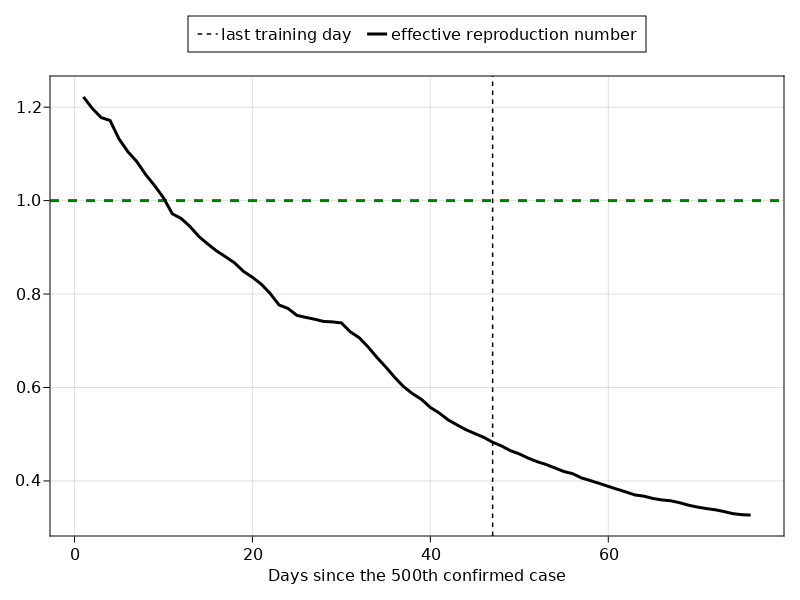
\includegraphics[width=\linewidth]{fb2/maricopa_az/20211216193717.fbmobility2.maricopa_az.R_effective.png}
        \end{subfigure}
        \begin{subfigure}[b]{0.4\linewidth}
            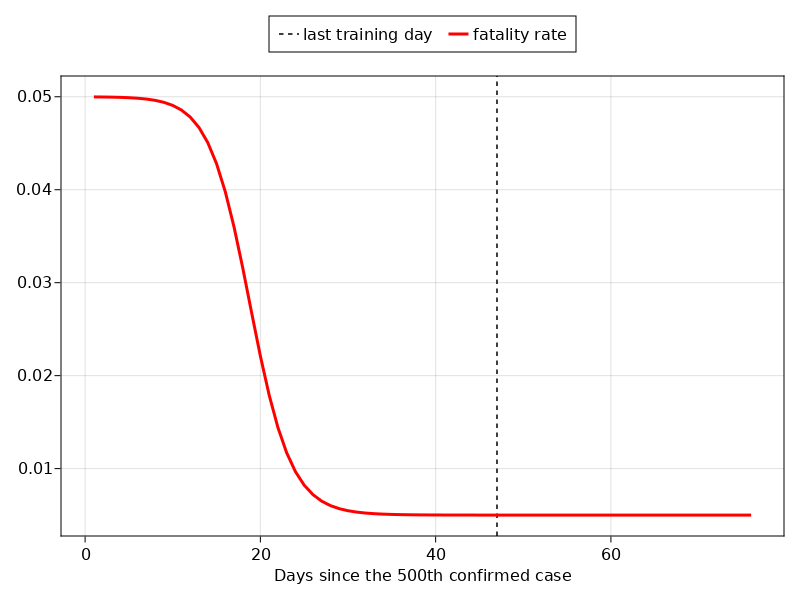
\includegraphics[width=\linewidth]{fb2/maricopa_az/20211216193717.fbmobility2.maricopa_az.fatality_rate.png}
        \end{subfigure}
        \subcaption{3rd. version}
    \end{subfigure}

    \caption{The effective reproduction number and the fatality rate for Maricopa (Arizona) learned by different versions of the model}
    \label{fig:R0-and-fatality-marico}
\end{figure}
